\documentclass{article}%
\usepackage[T1]{fontenc}%
\usepackage[utf8]{inputenc}%
\usepackage{lmodern}%
\usepackage{textcomp}%
\usepackage{lastpage}%
\usepackage{authblk}%
\usepackage{graphicx}%
%
\title{Regulation of MYC Expression and Differential JQ1 Sensitivity in Cancer Cells}%
\author{Shelby Proctor}%
\affil{Blood Transfusion Centre of Slovenia, Ljubljana, Slovenia}%
\date{01{-}01{-}2013}%
%
\begin{document}%
\normalsize%
\maketitle%
\section{Abstract}%
\label{sec:Abstract}%
While imaging or modulating the cells affects the outcome of current interventions, researchers at Stanford University have successfully induced specific inducible activation by a low{-}level laser{-}based laser to produce a complete, genetic response to the patient's stem cell tissue.\newline%
The study demonstrates that such artificial activation is likely to lead to extensive and improved therapeutic response in mouse models of Focal Cerebral Inducible Inhibition (FCII), a medical term for the conversion of axons and cell structures lost during use of plasmapheresis (heart surgery) to spinal cord regeneration in rats.\newline%
FCII in rats is a condition that causes long{-}term mental illness and paralysis by rerouting axons and cell structures lost during use of plasmapheresis during the heart or spinal cord.\newline%
Focal Cerebral Inhibition involves a process by which nerve fibers lose axons and cell structures to transfer information to other nerve cells. In injected cells, this loss is not immediate, thus allowing for early response to therapies.\newline%
For example, Harvard Medical School researchers demonstrated in the 1990s that peptide{-}based implanting procedures for post{-}operative nerve grafts, with the donor's own replacement nervous system, successfully resulted in the regeneration of autonomic nervous system axons on rats and, in 2008, the natural regenerative response of that therapy became the subject of a highly successful, federally{-}funded phase{-}two clinical trial.\newline%
The new finding, published in the journal Cell Stem Cell, in conjunction with colleagues from the Heidelberg Institute for Laboratory Research in Germany, is the first mouse model in which such rejection of specialized, regular IV{-}provider translocation into the critical tissue of the affected limb spleen (embryo of a leg severed during heart surgery) occurs.\newline%
The laboratory results indicate the plasticity of adenovirus cells, precursor to specialized types of human heart and peripheral blood vessels, as well as of transcription factors, such as transcriptional dystrophin, that modify the injury site and activate the limb{-}like processing of area of formation, which in turn also remains activated during therapy.\newline%
"This human study results in the provision of an idealized proof{-}of{-}concept mouse model for the importance of loss of axons in Focal Cerebral Inducible Inhibition," said Jiyeun Han, associate professor of medicine in the department of Cell and Developmental Biology at Stanford and senior author of the study. "We hope that with new exploratory therapies, such as AP cells in tissue{-}replacement trial, we might discover a way of reducing long{-}term risk of Focal Cerebral Inducible Inhibition and advanced research in the area is likely to develop other more common pathways implicated in the syndrome, including pain signaling in animals. Only a small number of drugs with these effects have been studied at this stage, and we hope that the success of this study points the way toward more advanced therapies."

%
\subsection{Image Analysis}%
\label{subsec:ImageAnalysis}%


\begin{figure}[h!]%
\centering%
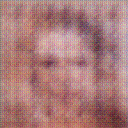
\includegraphics[width=150px]{500_fake_images/samples_5_384.png}%
\caption{A Close Up Of A Small Bird In A Field}%
\end{figure}

%
\end{document}